\documentclass[
	a4paper,
	11pt,
	twoside,
	DIV=12,
	BCOR=15mm,
	abstracton,
	parskip,
	listof=totoc,
	bibliography=totoc]{scrreprt}

% Headers and Footers
\pagestyle{headings}

% Font as serif
\setkomafont{disposition}{\normalcolor\bfseries}

\usepackage[utf8]{inputenc}
\usepackage[english]{babel}

\usepackage[numbers]{natbib}
\bibliographystyle{plainnat}
\usepackage[printonlyused]{acronym}

\usepackage{url}
\usepackage{hyperref}

\usepackage{graphicx}
\usepackage{rotating}
\usepackage{subcaption}

\usepackage{todo}

% Listings
\usepackage{scrhack}
\usepackage{listings}
\lstset{
	numbers=left,
	numbersep=5pt,
	xleftmargin=2em,
	xrightmargin=1em,
	framexleftmargin=1em,
	frame=tb,
	captionpos=b}
\lstset{
	basicstyle=\ttfamily\footnotesize}

% Quotes before Chapter
\usepackage{epigraph}
\setlength{\epigraphwidth}{.6\textwidth}
\setlength{\epigraphrule}{0pt}

% Hurenkinder und Schusterjungen
\clubpenalty = 10000
\widowpenalty = 10000
\displaywidowpenalty = 10000

% Line Spacing Table
\renewcommand{\arraystretch}{1.6}

\begin{document}

\pagenumbering{roman}

\subject{
	Master Thesis}
\title{
	Self-adaptation??? in Programmable Automation Controllers based on Hybrid
	Multicores}
\author{
	Christoph Rüthing\\[-12pt]
	Student ID: 6619350}
\publishers{
	{\large Supervisors}\\[12pt]
	Prof. Dr. Marco Platzner\\
	Dipl.-Inf. Andreas Agne}
\lowertitleback{
	Master Thesis\\
	\textbf{
		Self-adaptation in Programmable Automation Controller\\
		based on Hybrid Multicores}\\[.5cm]
	University of Paderborn\\
	Faculty of Electrical Engineering, Computer Science and Mathematics\\
	Department of Computer Science\\
	Warburger Str. 100\\
	33098 Paderborn}

\maketitle

\cleardoublepage

%!TEX root = thesis.tex
\begin{abstract}
Modern industrial applications include a broad range of requirements, far
exceeding the traditional control and automation tasks. To accomodate these
new challenges, the so-called \ac{PAC} was introduced, combining the
advantages of traditional \acp{PLC} and \acp{PC}. The recent versions,
additionally, incorporate custom hardware for high-performance or low-latency
tasks, implemented on an \ac{FPGA}. The goal of this master project is to
develop an adaptive PAC, based on a heterogeneous reconfigurable
hardware/software architecture (ReconOS), with a focus on communication,
programmability and self-adaption strategies.
\end{abstract}

\chapter*{Declaration}

I hereby declare that I prepared this thesis entirely on my own and have not
used outside sources without declaration in the text. Any concepts or
quotations applicable to these sources are clearly attributed to them. This
thesis has not been submitted in the same or substantially similar version,
not even in part, to any other authority for grading and has not been
published elsewhere.\\[27pt]

\begin{center}
	\begin{tabular}{l p{0.1\textwidth} r}
		\cline{1-1}\cline{3-3}
		\begin{minipage}[t]{0.4\textwidth}
			\centering
			City, Date
		\end{minipage}
		&
		\begin{minipage}[t]{0.2\textwidth}
		\end{minipage}
		&
		\begin{minipage}[t]{0.4\textwidth}
  			\centering
  			Signatur
		\end{minipage}
	\end{tabular}
\end{center}

\tableofcontents
\listoffigures
\listoftables
%!TEX root = thesis.tex
\chapter*{List of Abbreviations}
\begin{acronym}
\acro{PAC}{Programmable Automation Controller}
\acro{PLC}{Programmable Logic Controller}
\acro{FPGA}{Field Programmable Gate Array}
\acro{CTOS}{commercial off-the-shelf}
\acro{CPU}{Central Processing Unit}
\acro{GPU}{Graphics Processing Unit}
\acro{DSP}{Digital Signal Processor}
\acro{PC}{Personal Computer}
\acro{ARC}{Automation Research Company}
\acro{COTS}{commercial off-the-shelf}
\acro{ASIC}{Application-Specific Integrated Circuit}
\acro{VHDL}{Very High Speed Integrated Circuit Hardware Description Language}
\acro{HDL}{Hardware Description Language}
\acro{SoC}{System on Chip}
\acrodefplural{SoC}[SoCs]{Systems on Chip}
\acro{HLS}{High Level Synthesis}
\acro{OS}{Operating System}
\acro{OSFSM}{Operating System Synchronization Finite State Machine}
\acro{OSIF}{Operating System Interface}
\acro{MEMIF}{Memory Interface}
\acro{POSIX}{Portable Operating System Interface}
\acro{TLB}{Translation Look-aside Buffer}
\acro{MMU}{Memory Management Unit}
\acro{RTL}{Register Transfer Level}
\acro{ISPS}{Instruction Set Processor Specification}
\acro{CMU-DA}{Carnegie-Mellon University Design Automation}
\acro{IP}{Intellectual Property}
\acro{RAM}{Random Access Memory}
\acro{FIFO}{First In First Out}
\acro{AXI}{Advanced eXtensible Interface Bus}
\acro{FSM}{Finite State Machine}
\acro{DSP}{Digital Signal Processor}
\acro{API}{Application Programming Interface}
\acro{RDK}{ReconOS Development Kit}
\acro{Tcl}{Tool Command Language}
\acro{LUT}{Lookup-Table}
\acro{MSB}{most significant bit}
\acro{LSB}{least significant bit}
\acro{6DoF}{six Degrees of Freedom}
\acro{CNC}{Computer Numerical Control}
\acro{CAD}{Computer Aided Design}
\acro{ITO}{Indium Tin Oxide}
\acro{ADC}{Analog-Digital-Converter}
\acro{SPI}{Serial Peripheral Interface}
\acro{Pmod}{Peripheral Module}
\acro{PID}{Proportional Integral Derivative}
\acro{PWM}{Pulse-Width Modulation}
\acro{IC}{Integrated Circuit}
\acro{I2C}[I\textsuperscript{2}C]{Inter-Integrated Circuit}
\acro{PID}{Proportional-Integral-Derivative}
\end{acronym}

\cleardoublepage

\pagenumbering{arabic}

%!TEX root = thesis.tex
\chapter{Introduction}
%\epigraphhead[60]{\epigraph{``The future for PACs hinges on the incorporation
%of embedded technology''}{\textit{\citet{bel05}}}}

Modern industrial applications include a broad range of requirements, far
exceeding the traditional control and automation tasks. Buzzwords like
\emph{Industry 4.0} or the \emph{Internet of Things} emphasize the growing
demand of features. While a typical control system interfaces with simple
sensors and actuators, modern applications require more sophisticated features
like network connectivity, integration into enterprise systems or device
interoperability. To accommodate these new challenges and since the nowadays
dominating \ac{PLC} reaches its limits, the \ac{PAC} was introduced as the
next generation of control. It combines the reliability and robustness of a
\ac{PLC} with the advanced software capabilities of a \ac{PC}. By
incorporating state-of-the-art embedded technology like \acp{FPGA} and its
integration with general purpose processors on a single chip, these devices
eliminate the need for an expensive custom hardware and allow  the use of
\ac{CTOS} components, without loosing the benefits of executing time critical
control functions directly in silicon.

Unfortunately, the increasing complexity of such systems introduces new
challenges and demand convenient programming methods abstracting the
underlying low-level components, to make these devices accessible to a broad
range of developers. Classical ladder logic used for \acp{PLC} reaches its
limits and \ac{FPGA} technology is restricted to hardware designers capable of
handling low level programming languages like \ac{VHDL}. Because of its
acceptance in the field of software engineering and its eligibility to model
embedded systems composed of concurrently running tasks, the multithreaded
approach seems to be suitable as a convenient programming model for these
hybrid devices. The different threads specified by the developer are
distributed across the system's \ac{CPU} and \ac{FPGA} resources and
communicate via defined interaction mechanisms like message passing or shared
memory.\todo{Proposal Andreas}
\begin{itemize}
\item Develop a reconfigurable infrastructure for direct communication
between hardware threads. The new communication method should be integrated
into the ReconOS programming model as a new or as an extension of an existing
operating system abstraction. The choice of communication method should be
made by the runtime system in a way that is transparent for the programmer of
the hardeware thread.
\item Develop a toolchain that enables the use of \ac{HLS} for the creation of
ReconOS hardware threads. Investigate, how \ac{HLS} can be used to generate
the processing logic of a thread as well as the \ac{OSFSM}.
\item Implement a method to meassure the power consumption of the system.
Investigate means to meassure the on-chip power usage in a fine-grained way.
Investigate whether it is possible to meassure the power usage of individual
hardware threads.
\item Develop a \ac{PAC} that controlls a ball-on-plate application. The
application should contain components for the tracking of the ball, inverse
kinematics, and the required control algorithms. These components should be
implemented as a combination of hardware and software threads.
\item Use the previously developed application and components to meassure
thread performance, resource utilization and power consumption. Make the
application adapt to given goals and constraints by mechanisms like switching
on and off hardware and software threads, or switching between different
algorithms or implementations. Investigate different adaptation strategies
ranging from simple heuristics to more sophisticated methods involving machine
learning.
\end{itemize}
\chapter{Background}
\section{Programmable Automation Controllers}
\begin{itemize}
\item What is an PAC
\item Differentiation to PLC and PC
\item Incorporation of FPGAs
\item Problems (Hard to program, error-prone, ...)
\end{itemize}
\section{ReconOS}
\begin{itemize}
\item Multithreaded Programming model
\item Abstraction form hardware software boundary
\item ...
\end{itemize}

\chapter{Interconnect}
\begin{itemize}
\item Motivation for interconnect (experiments, other projects, ...)
\item Always via software to slow
\item Consideration (resource limitations, ...)
\item Reconfigurable later on?
\end{itemize}
\section{Architectural Considerations}
\begin{itemize}
\item Comparison of different approaches
\item HThreads, ...?
\end{itemize}
\section{Implementation}
\section{Evaluation}
\begin{itemize}
\item measure time differences for old/new
\item show speedup/speeddown
\end{itemize}

\chapter{Integration of HLS}
\begin{itemize}
\item Motivation of HLS
\end{itemize}

\chapter{Demonstrator}

\cleardoublepage

\bibliography{thesis}

%!TEX root = thesis.tex
\chapter{Appendix}
\section{Evaluation of \acs{PID} Controller}
Although the scope of this thesis does not focuses on controller design and
tuning, a brief evaluation of the implemented \ac{PID} controller is given in
this section. By systematically exploring different values for the
\ac{PID} parameters, the final system applies $K_P = -0.09$, $K_I = 0$ and
$K_D = -28$. Figure \ref{fig:demo_pid} shows a tracking of the ball for two
applications.
\begin{figure}
	\centering
	\begin{subfigure}{0.49\textwidth}
		\centering
		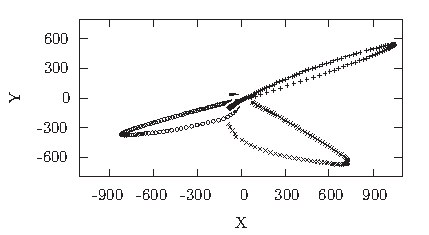
\includegraphics[width=\textwidth]{../figures/eval_pos}
		\caption{Balancing of ball in the center}
		\label{fig:eval_pos}
	\end{subfigure}
	\begin{subfigure}{0.49\textwidth}
		\centering
		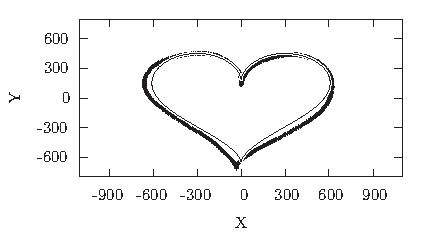
\includegraphics[width=\textwidth]{../figures/eval_traj}
		\caption{Following of a fixed trajectory}
		\label{fig:eval_traj}
	\end{subfigure}
	\caption{Captures of ball's movement controlled by \acs{PID} controller}
	\label{fig:demo_pid}
\end{figure}
For figure \ref{fig:eval_pos} the ball is balanced at the center of the plate
and any external disturbance is compensated, with the aim to keep the ball on
the plate. The figure shows a slight overshoot at the center and, due to a
missing integral term, never reaches the absolute center. Since the ball has a
relatively high initial friction, a large angle is needed to give the ball an
initial impulse. It then destabilizes and never reaches a resting position.
Therefore, a small inaccuracy for its final position is acceptable.
Additionally to the balancing of the ball in the center, figure
\ref{fig:eval_traj} shows an exemplary trajectory for the ball to follow.
Again, an inaccuracy from the desired trajectory in the direction of movement
is apparent. The trajectory is achieved by changing the target position of the
ball over time and adjusting the \ac{PID} controller to avoid the so-called
derivative kick.

\end{document}